\documentclass[journal]{IEEEtran}

\usepackage[T1]{fontenc}
\usepackage[utf8]{inputenc}
\usepackage{amsmath,amssymb,amsfonts}
\usepackage{graphicx}
\usepackage{booktabs}
\usepackage{array}
\usepackage{url}
\usepackage{xcolor}
\usepackage[hidelinks]{hyperref}
\usepackage{orcidlink}
\usepackage{balance}

\graphicspath{{../figures/}}

\renewcommand{\topfraction}{0.92}
\renewcommand{\bottomfraction}{0.75}
\renewcommand{\textfraction}{0.08}
\renewcommand{\floatpagefraction}{0.80}

% IEEEtran hard-codes an em-dash after the abstract and index-terms names; the CAOS
% content standard (ADR-0067) excludes em-dashes, so the separator is a full stop.
\makeatletter
\def\abstract{\normalfont
    \if@twocolumn
      \@IEEEabskeysecsize\bfseries\textit{\abstractname}.\ \relax
    \else
      \bgroup\par\addvspace{0.5\baselineskip}\centering\vspace{-1.78ex}\@IEEEabskeysecsize\textbf{\abstractname}\par\addvspace{0.5\baselineskip}\egroup\quotation\@IEEEabskeysecsize
    \fi\@IEEEgobbleleadPARNLSP}
\def\IEEEkeywords{\normalfont
    \if@twocolumn
      \@IEEEabskeysecsize\bfseries\textit{\IEEEkeywordsname}.\ \relax
    \else
      \bgroup\par\addvspace{0.5\baselineskip}\centering\@IEEEabskeysecsize\textbf{\IEEEkeywordsname}\par\addvspace{0.5\baselineskip}\egroup\quotation\@IEEEabskeysecsize
    \fi\@IEEEgobbleleadPARNLSP}
\makeatother

% Page-1 header block (conventions/manuscript-header-standard.md). The four document
% macros are set by the publishing tool when the version DOI is reserved.
\newcommand{\doctype}{Technical report}
\newcommand{\docversion}{v1.1}
\newcommand{\docdate}{18 September 2026}
\newcommand{\versiondoi}{10.5281/zenodo.22824781}
\newcommand{\conceptdoi}{10.5281/zenodo.21519794}
\newcommand{\docrepo}{github.com/fsantibanezleal/CAOS\_RES\_Maqueta}
\newcommand{\headerblock}{%
\begin{center}
\fbox{\parbox{0.94\textwidth}{\small\raggedright
\textbf{\doctype} \quad$\cdot$\quad \docversion, \docdate \quad$\cdot$\quad Licence CC BY 4.0\\[2pt]
CAOS open-research programme \quad$\cdot$\quad CAOS\_RES\_Maqueta, open-data 3D reconstruction of real places\\[2pt]
Version DOI \href{https://doi.org/\versiondoi}{\texttt{\versiondoi}} \quad$\cdot$\quad
concept DOI (always latest) \href{https://doi.org/\conceptdoi}{\texttt{\conceptdoi}}\\[2pt]
Not peer reviewed. Source code, data and computational records: \href{https://\docrepo}{\texttt{\docrepo}}
}}
\end{center}}

\begin{document}

\title{Maqueta: Height Provenance in Open-Data\\ 3D Urban Reconstruction Across 118 Places}

\author{Felipe~Santiba\~nez-Leal~\orcidlink{0000-0002-0150-3246}%
\thanks{F. Santiba\~nez-Leal is with the CAOS open-research programme, Santiago, Chile
(e-mail: fsantibanez@gmail.com; ORCID 0000-0002-0150-3246).}%
\thanks{Interactive tool and reproducible pipeline (MIT) at
\url{https://github.com/fsantibanezleal/CAOS_RES_Maqueta}; the \texttt{geoscena} fusion core at
\url{https://github.com/fsantibanezleal/CAOS_GeoScena}.}}

% The leading {} lets IEEEtran's \MakeUppercase reach \doctype, so the whole head is set in capitals.
\markboth{{}\doctype\ \docversion, 2026}%
{Santiba\~nez-Leal: Height provenance in open-data 3D urban reconstruction}

\IEEEaftertitletext{\vspace{-0.6\baselineskip}\headerblock\vspace{0.2\baselineskip}}

\maketitle

\begin{abstract}
A 3D city model is only as accurate as its building heights, and a model built from open data mostly infers those
heights, from a mapped floor count, a height raster or a default value, rather than taking them from a mapped
height. Maqueta reconstructs real places from open geospatial layers, with terrain from the Copernicus GLO-30
surface model, building footprints and roads from Overture Maps, water, green areas and rail from OpenStreetMap,
population from GHS-POP, and building heights from the Google Open Buildings 2.5D raster where it has coverage, and
it records for every building how its height was obtained. Across the $118$ baked places and $4.05$ million
buildings, $8.8\%$ of heights come from a mapped height attribute, $6.4\%$ from a mapped floor count, $73.2\%$ from
the Open Buildings 2.5D height raster, itself a model estimate from satellite imagery, and $11.6\%$ from a default
prior of $8$~m. A public LoD2 reference exists for two of the places, both in the Netherlands, where the raster has no
coverage. Against the 3D BAG, the fused heights have a root-mean-square error of $3.1$~m at Delft, with a bias of
$-0.1$~m, and of $8.3$~m at Amsterdam, with a bias of $-6.6$~m; the Amsterdam figure rests on $50$ reference
buildings. The raster heights, which supply most of the buildings, are not validated by this benchmark, and public
ground truth for open-data building heights is scarce.
\end{abstract}

\begin{IEEEkeywords}
3D city models, geospatial data fusion, building height, LoD2, open data, data provenance, OpenStreetMap, Google
Open Buildings.
\end{IEEEkeywords}

\section{Introduction}

\IEEEPARstart{A} 3D city model is used for solar-potential studies, flood and wind simulation, visibility and
noise analysis, and urban planning~\cite{biljecki15}, and every one of those uses depends on the building heights.
Authoritative models at level of detail~2 (LoD2), reconstructed from airborne lidar, exist for a handful of
well-mapped countries~\cite{peters}. For most of the world the heights are not surveyed: they are estimated from
attributes such as a floor count, from a height raster, or from a default value, and generating 3D city models
without elevation data is a matter of such estimation~\cite{biljecki17}. When a single-source extrusion is rendered
as a 3D city, nothing in the model distinguishes an estimated height from a mapped one.

Maqueta is a multi-source fusion tool that reconstructs an area from open layers, each carrying its source, licence,
release and fetch date, and it records for every building how its height was obtained. The provenance is read here
across the $118$ baked places, and the heights are benchmarked where an authoritative LoD2 reference exists. The
contribution is the per-building height provenance and its measurement across the places, not a new reconstruction
algorithm.

\section{Sources and the Height Ladder}\label{sec:method}

\emph{Layers.} Terrain comes from the Copernicus GLO-30 surface model~\cite{copdem}, building footprints and roads from
Overture Maps~\cite{overture}, which conflates OpenStreetMap, national mapping agencies and machine-learned
roofprints, water, green areas and rail from OpenStreetMap~\cite{osm}, and population from the GHS-POP R2023A
grid~\cite{ghspop}. The layers present depend on the place (Table~\ref{tab:layers}): every place has terrain, $116$
have population, $100$ have buildings and roads, $23$ to $26$ have the OpenStreetMap context layers, and the $18$
places without buildings, landscapes and heritage sites such as the Grand Canyon, Machu Picchu and the Chuquicamata
mine, have terrain and, at $16$ of them, population. The two Dutch places add
the LoD2 reference of the 3D BAG~\cite{peters} as a layer of its own.

\begin{table}[!t]
\centering
\caption{Layers of the $118$ baked places: the number of places that carry each layer.}
\label{tab:layers}
\footnotesize
\begin{tabular}{@{}l l r@{}}
\toprule
Layer & Source & Places \\
\midrule
Terrain & Copernicus GLO-30 & $118$ \\
Population & GHS-POP R2023A & $116$ \\
Buildings, roads & Overture Maps & $100$ \\
Green areas & OpenStreetMap & $26$ \\
Water & OpenStreetMap & $24$ \\
Rail & OpenStreetMap & $23$ \\
LoD2 reference & 3D BAG & $2$ \\
\bottomrule
\end{tabular}
\end{table}

\emph{Height ladder.} Each building footprint takes its height from the first of four rungs that yields a positive
value, and the rung is recorded with the building: (1) a mapped \texttt{height} attribute in Overture or
OpenStreetMap, used directly; (2) a mapped \texttt{num\_floors} attribute, multiplied by $3.2$~m; (3) the Google Open
Buildings 2.5D height raster, sampled at the footprint where the raster has coverage (Latin America, Africa, and
South and Southeast Asia); and (4) a default prior of $8$~m. Heights are clipped below at $2.5$~m. The raster is a
model estimate from Sentinel-2 imagery, for which its producers report a mean absolute error of
$1.5$~m~\cite{sirko23}; only the first rung is a mapped value, and none is a survey measurement made for this work.

\section{Height Provenance Across 118 Places}\label{sec:provenance}

\begin{figure}[!t]
\centering
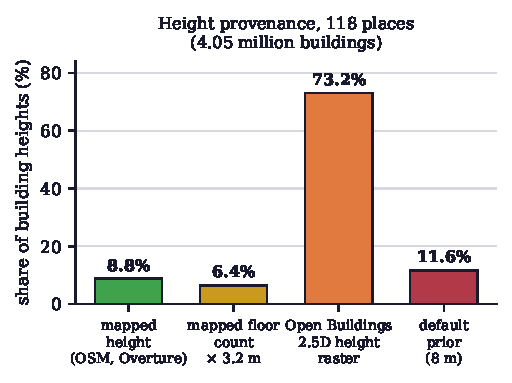
\includegraphics[width=\columnwidth]{fig-provenance.pdf}
\caption{Height provenance of the $4.05$ million buildings of the $118$ baked places: $8.8\%$ from a mapped height
attribute, $6.4\%$ from a mapped floor count, $73.2\%$ from the Open Buildings 2.5D height raster and $11.6\%$ from
the default prior.}
\label{fig:provenance}
\end{figure}

Over the $4.05$ million buildings of the $118$ places (Fig.~\ref{fig:provenance}), $8.8\%$ of heights come from a
mapped height attribute, $6.4\%$ from a mapped floor count, $73.2\%$ from the Open Buildings 2.5D raster and
$11.6\%$ from the default prior: more than nine in ten heights are estimated rather than mapped. The mix varies
strongly between places, and the global shares depend on which places were baked. The raster is the dominant rung at
$62$ of the $100$ places with buildings and is not used at $35$ of them; a few large Latin American
places carry most of its share, among them Buenos Aires ($98.7\%$ of $223$ thousand buildings) and Santiago
($93.9\%$ of $179$ thousand). Where the raster has no coverage, the prior can dominate, as in Tokyo ($91.5\%$), and
where mapped heights are abundant they dominate instead, as in New York ($99.3\%$) and S\~ao Paulo ($87.5\%$). At the
median place with buildings, $0.3\%$ of heights are mapped. Because the rung is recorded per building, a downstream
user can filter or weight each height by how it was obtained.

\section{Benchmark Where a LoD2 Reference Exists}\label{sec:benchmark}

\begin{figure}[!t]
\centering
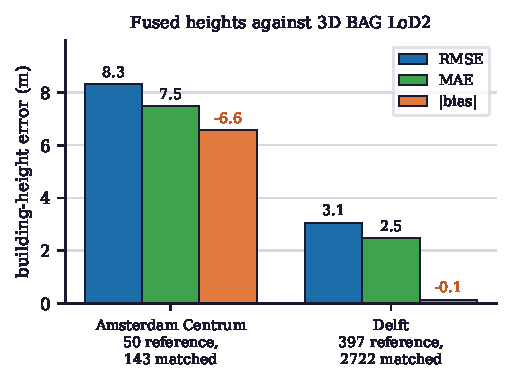
\includegraphics[width=\columnwidth]{fig-benchmark.pdf}
\caption{Fused-height error against the 3D BAG LoD2 reference at the two places that have one. Each fused building is
matched to the nearest reference building within $25$~m. Root-mean-square error $3.1$~m at Delft (bias $-0.1$~m;
$2722$ fused buildings matched to $397$ reference buildings) and $8.3$~m at Amsterdam (bias $-6.6$~m; $143$ matched to
$50$).}
\label{fig:benchmark}
\end{figure}

The 3D BAG reconstructs LoD2 models of all buildings in the Netherlands from lidar~\cite{peters}, and it gives the
reference height as the median roof height minus the ground level. Two of the $118$ places, Delft and Amsterdam
Centrum, lie in its coverage (Fig.~\ref{fig:benchmark}). Each fused building is matched by its centroid to the nearest
reference building within $25$~m, so several fused footprints can share one reference building, and the error is taken
over the matched fused buildings. At Delft, $2722$ fused buildings ($17.1\%$ of the place) match $397$ reference
buildings, with a root-mean-square error of $3.1$~m, a mean absolute error of $2.5$~m and a bias of $-0.1$~m. At
Amsterdam, $143$ fused buildings ($1.0\%$ of the place) match $50$ reference buildings, with $8.3$~m, $7.5$~m and a bias
of $-6.6$~m. The heights of both places come almost entirely from floor counts and the default prior, since the raster
does not cover
Europe: $41\%$ floor counts and $59\%$ prior at Delft, $7\%$ and $92\%$ at Amsterdam. The larger error and the low bias
at Amsterdam are consistent with the $8$~m default lying below the typical height of the matched buildings, although
two places, one of them with $50$ reference buildings, cannot establish that relation. Neither place contains a
raster height, so the rung that supplies $73.2\%$ of all heights is not validated by this benchmark.

\section{Discussion and Scope}\label{sec:discuss}

An open-data 3D city model is mostly estimated: in these $118$ places fewer than one building height in ten comes from
a mapped value, and most come from a height raster that is itself a model output. Recording the rung per building
makes that visible and lets a user treat a mapped height and a default differently. The validation is thin. Public
LoD2 references cover two of the places, both in a country without raster coverage, so they test the floor-count and
prior rungs only, and the Amsterdam estimate rests on $50$ reference buildings. The global shares describe this set of
places and would change with a different selection. The reconstructed scenes serve visualisation, teaching and
planning context, not survey-grade modelling. The reusable fusion core, \texttt{geoscena}, turns an area of interest
into a provenance-tracked scene bundle, and the product pipeline bakes a curated registry of places on top of it.

\section{Conclusion}

Maqueta reconstructs $118$ real places from open geospatial layers and records the provenance of every building
height. Of $4.05$ million heights, $8.8\%$ come from a mapped height attribute, $6.4\%$ from a mapped floor count,
$73.2\%$ from the Google Open Buildings 2.5D height raster and $11.6\%$ from a default prior. Where a public LoD2
reference exists, at two Dutch places, the fused heights have a root-mean-square error of $3.1$ and $8.3$~m; those
places test only the floor-count and prior rungs, and public ground truth for open-data building heights remains
scarce.

\appendices
\section{Reproduction}\label{app:repro}

The repository benchmark (\path{data/derived/benchmark.json}) carries, per place, the layer count, the triangle and
size totals, the height-provenance counts per rung and, where a LoD2 reference exists, the matched counts, the
root-mean-square error, the mean absolute error and the bias. Each place's manifest
(\path{data/derived/<place>/manifest.json}) records every layer's source, URL, licence, release, fetch date and
method. The figure script under \path{manuscripts/geo-reconstruction/figures/} reads \path{mq.json} in the data folder
beside it, a copy of the benchmark figures. The \texttt{geoscena} fusion core and the product pipeline
(\path{data-pipeline/}) rebuild a place from the recorded source releases; newer releases of the open sources change
the result. The open layers are fetched under their own licences and are not redistributed.

\balance

\begin{thebibliography}{00}

\bibitem{biljecki15} F.~Biljecki, J.~Stoter, H.~Ledoux, S.~Zlatanova, and A.~\c{C}\"oltekin, ``Applications of 3D
city models: State of the art review,'' \emph{ISPRS International Journal of Geo-Information}, vol.~4, no.~4,
pp.~2842--2889, 2015. doi:10.3390/ijgi4042842.

\bibitem{biljecki17} F.~Biljecki, H.~Ledoux, and J.~Stoter, ``Generating 3D city models without elevation data,''
\emph{Computers, Environment and Urban Systems}, vol.~64, pp.~1--18, 2017.
doi:10.1016/j.compenvurbsys.2017.01.001.

\bibitem{peters} R.~Peters, B.~Dukai, S.~Vitalis, J.~van~Liempt, and J.~Stoter, ``Automated 3D reconstruction of
LoD2 and LoD1 models for all 10 million buildings of the Netherlands,'' \emph{Photogrammetric Engineering \&
Remote Sensing}, vol.~88, no.~3, pp.~165--170, 2022. doi:10.14358/PERS.21-00032R2.

\bibitem{sirko23} W.~Sirko \emph{et al.}, ``High-resolution building and road detection from Sentinel-2,'' 2023.
arXiv:2310.11622.

\bibitem{copdem} European Space Agency, ``Copernicus Digital Elevation Model (GLO-30),'' 2021.
doi:10.5270/ESA-c5d3d65.

\bibitem{ghspop} M.~Schiavina, S.~Freire, and K.~MacManus, ``GHS-POP R2023A: GHS population grid multitemporal
(1975--2030),'' European Commission, Joint Research Centre, 2023. doi:10.2905/2FF68A52-5B5B-4A22-8F40-C41DA8332CFE.

\bibitem{overture} Overture Maps Foundation, ``Overture Maps data: buildings and transportation themes,''
\url{https://overturemaps.org}.

\bibitem{osm} OpenStreetMap contributors, ``OpenStreetMap,'' \url{https://www.openstreetmap.org}.

\end{thebibliography}

\end{document}
